\documentclass{article}

\usepackage{../preamble}
\standalonetrue

\title{MATH 316 Lecture 8}
\author{Ashtan Mistal}
\date{May 25 2021}

\begin{document}

\ifstandalone
\maketitle
\fi

\graphicspath{{./Lecture08/}}

\section{Introduction}

\begin{itemize}
    \item Midterm is on Tuesday, June 8th 12:30 to 2pm. 
    \item Send an email (on Canvas), and explain if you have difficulties regarding the exam including timezone differences. 
    \item Homeworks can be on Webwork. For the weeks that we have Webwork homework, it will be \textbf{instead} of written work. 
    \item It will be a mixture of webwork homework and written homework for the rest of the course; one week could we webwork and the next could be written. 
\end{itemize}

\section{Recap of last lecture}

We covered two categories last week:

We discussed eigenvalue problems, or boundary value problems, of (P1, P2, P3), which had the following form:

$$y'' + \lambda y = 0$$

with different boundary conditions:

\begin{itemize}
    \item P1 are Dirichlet boundary conditions (Fourier sine series)
    \item P2 are Neumann boundary conditions (Fourier cosine series)
    \item P3 are periodic boundary conditions (Mixture of Fourier sine and cosine series)
\end{itemize}

\subsection{Fourier series}

A periodic function on $(-L, L)$ and integrable can be written as 

$$f(t) = \frac{a_0}{2} + \sum_{n = 1}^\infty a_n \cos(\frac{n \pi t}{L}) + \sum_{n = 1}^\infty b_n \sin(\frac{n \pi t}{L})$$

$a_0$ can be found through the following formula:

$$a_0 = \frac{1}{L} \int_{-L}^L f(t) dt$$

$a_n$ can be found through

$$a_n = \frac{1}{L} \int_{-L}^{L} f(t) \cos(\frac{n \pi t}{L}) dt$$

And $b_n$ can be found from:

$$b_n = \frac{1}{L} \int_{-L}^L f(t) \sin(\frac{n \pi t}{L}) dt$$

\subsection{Example 1 (Continued from last class)}

$$f(t) = \begin{matrix} t & -L \leq t < 0 \\ 0 & 0 \leq t < L \end{matrix}, f(t + 2L) = f(t)$$

$a_0 = \frac{-L}{2}$; $a_n = \frac{L}{n^2 \pi^2} \left(1 - \cos(n \pi ) \right) = \frac{L}{n^2 \pi^2} \left(1 - (-1)^n \right)$ for $n \in \NN$

\hfill

$b_n = \frac{1}{L} \int_{-L}^L f(t) \sin(\frac{n \pi t}{L}) dt =  \frac{1}{L} \int_{-L}^0 t \sin(\frac{n \pi t}{L}) dt$

Using integration by parts, we get the following:

$b_n = \left. \frac{L}{n \pi}\left( \cos(n \pi) - \underbrace{\frac{\sin(n \pi)}{n \pi}}_{ = 0} \right) \right.$

$b_n = \frac{L}{n \pi} \cos(n \pi) = \frac{L}{n \pi} (-1)^n$ for $n \in \NN$

Substitute $(a_0, a_n, b_n)$ into the equation: 

$$f(t) = \frac{a_0}{2} + \sum_{n = 1}^\infty a_n \cos(\frac{n \pi t}{L}) + \sum_{n = 1}^\infty b_n \sin(\frac{n \pi t}{L})$$

$$\Rightarrow f(t) = \frac{-L}{4} + L \sum_{n = 1}^\infty \frac{(1 - (-1)^n)}{n^2 \pi^2} \cos(\frac{n \pi t}{L}) +  L \sum_{n = 1}^\infty \frac{(-1)^n}{n \pi} \sin(\frac{n \pi t}{L})$$

If $L = \pi$:

$$f(t) = \frac{\pi}{4} + \sum_{n = 1}^\infty \frac{(1-  (-1)^n)}{n^2 \pi} \cos(n t) + \sum_{n = 1}^\infty \sin(n t)$$

\subsection{Example 2}

Fourier series example. 

$$f(t) = \begin{matrix} \left\{ \begin{matrix} -1 & -1 < t < 0 \\ 1 & 0 < t < 1 \end{matrix} \right. & f(t+2) = f(t) \end{matrix}$$

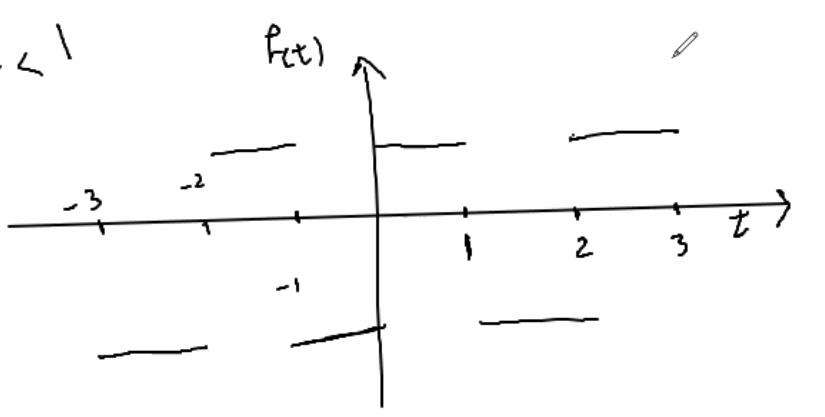
\includegraphics[width = 0.95 \textwidth]{image1.png}

This is a square wave function, and it is odd. 

$f_{odd}(x) \cdot f_{even} (x) = f_{odd} (x)$: An odd function multiplied by an even funciton is an odd function. 

$f_{odd} (x) \cdot f_{odd} (x) = f_{even} (x)$: An odd funciton multiplied by an odd function is an even function. 


If $f(t)$ is an even function:

$$\int_{-L}^L f(t) dt = 2 \int_0^L f(t) dt$$

If $f(t)$ is an odd function:

$$\int_{-L}^L f(t) dt = 0$$

Now, let's find out what the coefficients are of the fourier series. 

$$a_0 = \frac{1}{L} \int_{-L}^L \underbrace{f(t)}_{odd} dt = 0$$

$$a_n = \frac{1}{L} \int_{-L}^L \underbrace{f(t)}_{odd} \underbrace{\cos(\frac{n \pi t}{L})}_{even} dt = 0$$

(note that L = 1)

$$b_n = \int_{-1}^1 f(t) \sin(n \pi t) dt = 2 \int_{0}^{1} (1) \sin(n \pi t) dt = \left. - \frac{2}{n \pi} \cos(n \pi t) \right|_{0}^{1}$$

$$b_n = - \frac{2}{n \pi} \left( \cos(n \pi) - 1 \right) = \frac{4}{(2k - 1) \pi}, \text{with } n = 2k-1 \text{ for } k \in \NN$$

$$\Rightarrow f(t) = \sum_{k = 1}^\infty \frac{4}{(2k-1) \pi} \sin \left( (2k-1) \pi t \right) = \frac{4}{\pi} \sum_{k = 1}^\infty \frac{\sin \left( (2k-1) \pi t \right)}{2k-1}$$

\subsection{Example 2, part B}

$$f(t) = \begin{matrix} \left\{ \begin{matrix} -t & -2 < t < 0 \\ t & 0 \leq t \leq 2 \end{matrix} \right. & f(t+4) = f(t) \end{matrix} $$

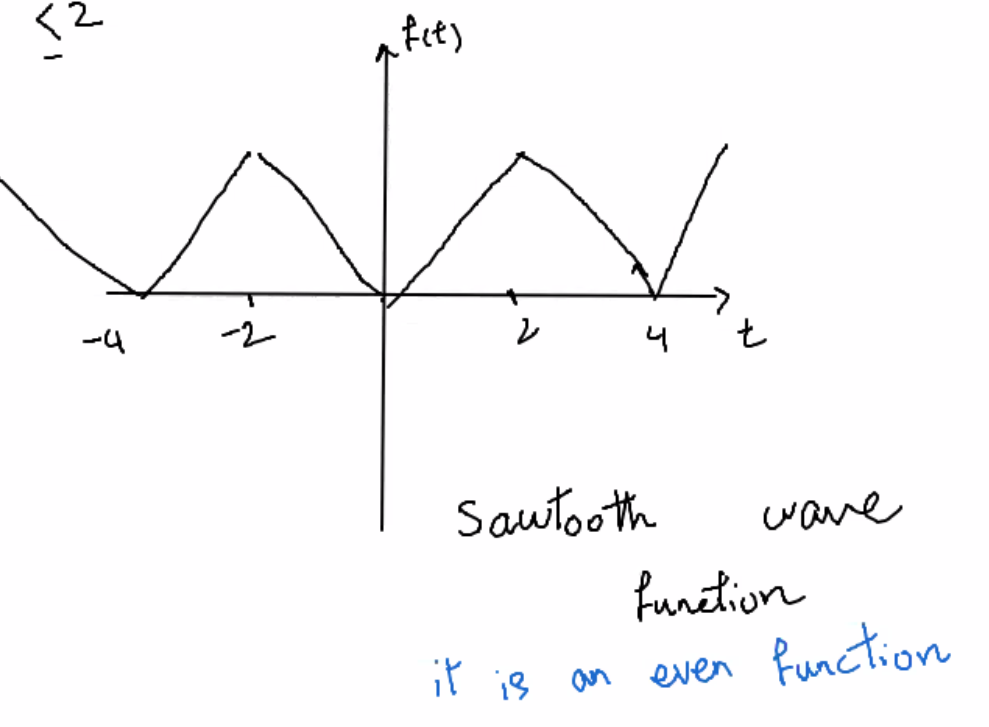
\includegraphics[width = 0.95 \textwidth]{image2.png}

[Note that this is a triangle wave, not a sawtooth wave, but it does not matter for the problem]

$$b_n = 0$$

$$a_0 = \frac{2}{2} \int_{0}^2 t dt = \left. \frac{t^2}{2} \right|_0^2 = 2$$

$$a_n = \frac{2}{L} \int_{0}^2 t \cos (\frac{n \pi t}{2}) dt$$

Using integration by parts, with the following:

$$\begin{matrix} u = t & dv = \cos(\frac{n \pi t}{2}) dt \\ du = dt & v = \frac{2}{n \pi} \sin(\frac{n \pi t}{2}) \end{matrix}$$

$$ = \underbrace{\left. \frac{2}{n \pi} t \sin(\frac{n \pi t}{2} ) \right|_0^2}_{ = 0} - \frac{2}{n \pi} \int_{0}^2 \sin(\frac{n \pi t}{2}) dt = \left. \frac{4}{n^2 \pi^2} \cos(\frac{n \pi t}{2}) \right|_0^2 = \frac{4}{n^2 \pi^2} (\cos(n \pi) - 1)$$

$$\Rightarrow a_n = \frac{-8}{(2k-1)^2 \pi^2}$$

(substituting $n = 2k-1$ above)

$$f(t) = 1 - \frac{8}{\pi^2} \sum_{k = 1}^\infty \frac{\cos \left( \frac{(2k-1) \pi t}{2} \right)}{(2k-1)^2}$$

\textbf{See slides; handwritten before page 6 and pages 6 up to 9 are covered in moderate depth(page numbers based on the numbers at the bottom of the page), and an overview up to the end. Example 3 is an exercise. The last slide is important.}

\section{Fourier Series Slides}

Included here for reference; also available on Canvas under Modules

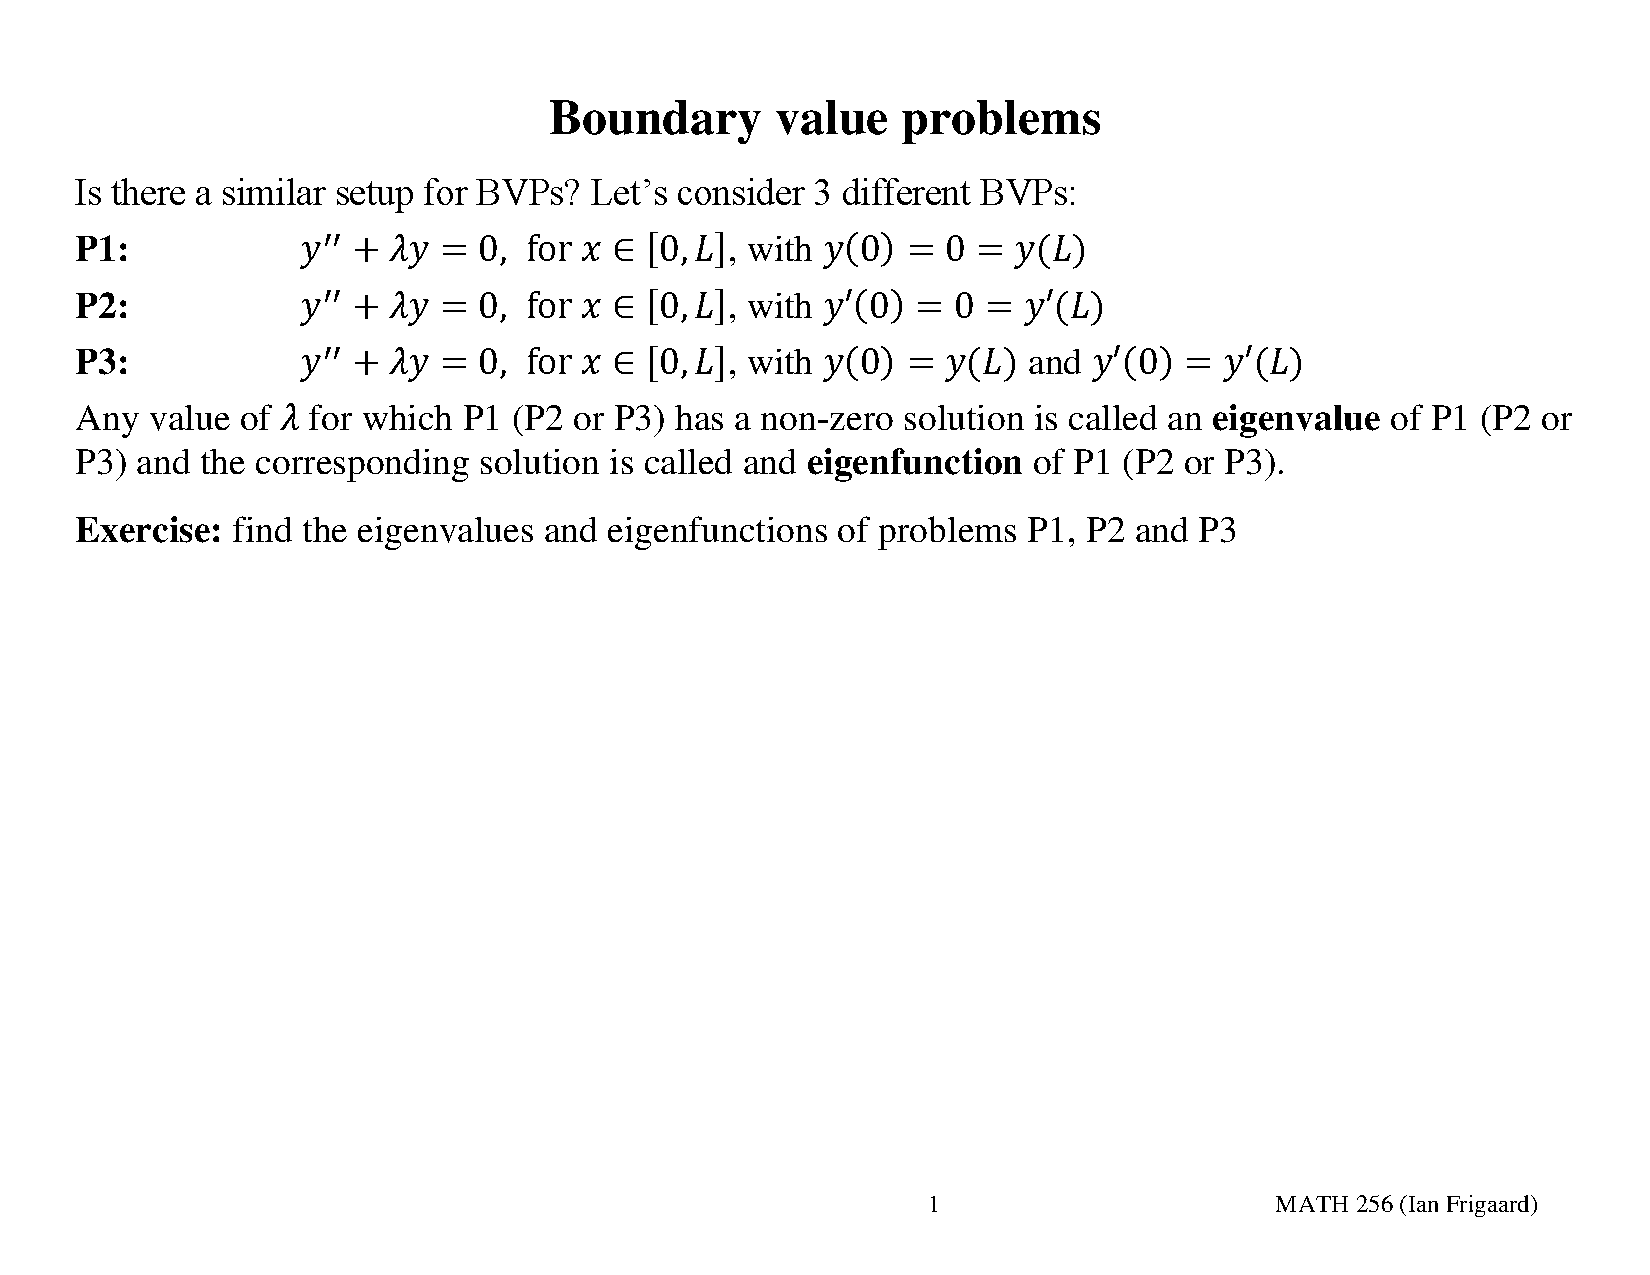
\includepdf[pages=-]{FourierSeries.pdf}

\end{document}

